\begin{figure}[tb]
  \centering
  \resizebox{\textwidth}{!}{\fontsize{10pt}{10pt}\selectfont% GNUPLOT: LaTeX picture with Postscript
\begingroup
  \makeatletter
  \providecommand\color[2][]{%
    \GenericError{(gnuplot) \space\space\space\@spaces}{%
      Package color not loaded in conjunction with
      terminal option `colourtext'%
    }{See the gnuplot documentation for explanation.%
    }{Either use 'blacktext' in gnuplot or load the package
      color.sty in LaTeX.}%
    \renewcommand\color[2][]{}%
  }%
  \providecommand\includegraphics[2][]{%
    \GenericError{(gnuplot) \space\space\space\@spaces}{%
      Package graphicx or graphics not loaded%
    }{See the gnuplot documentation for explanation.%
    }{The gnuplot epslatex terminal needs graphicx.sty or graphics.sty.}%
    \renewcommand\includegraphics[2][]{}%
  }%
  \providecommand\rotatebox[2]{#2}%
  \@ifundefined{ifGPcolor}{%
    \newif\ifGPcolor
    \GPcolorfalse
  }{}%
  \@ifundefined{ifGPblacktext}{%
    \newif\ifGPblacktext
    \GPblacktexttrue
  }{}%
  % define a \g@addto@macro without @ in the name:
  \let\gplgaddtomacro\g@addto@macro
  % define empty templates for all commands taking text:
  \gdef\gplbacktext{}%
  \gdef\gplfronttext{}%
  \makeatother
  \ifGPblacktext
    % no textcolor at all
    \def\colorrgb#1{}%
    \def\colorgray#1{}%
  \else
    % gray or color?
    \ifGPcolor
      \def\colorrgb#1{\color[rgb]{#1}}%
      \def\colorgray#1{\color[gray]{#1}}%
      \expandafter\def\csname LTw\endcsname{\color{white}}%
      \expandafter\def\csname LTb\endcsname{\color{black}}%
      \expandafter\def\csname LTa\endcsname{\color{black}}%
      \expandafter\def\csname LT0\endcsname{\color[rgb]{1,0,0}}%
      \expandafter\def\csname LT1\endcsname{\color[rgb]{0,1,0}}%
      \expandafter\def\csname LT2\endcsname{\color[rgb]{0,0,1}}%
      \expandafter\def\csname LT3\endcsname{\color[rgb]{1,0,1}}%
      \expandafter\def\csname LT4\endcsname{\color[rgb]{0,1,1}}%
      \expandafter\def\csname LT5\endcsname{\color[rgb]{1,1,0}}%
      \expandafter\def\csname LT6\endcsname{\color[rgb]{0,0,0}}%
      \expandafter\def\csname LT7\endcsname{\color[rgb]{1,0.3,0}}%
      \expandafter\def\csname LT8\endcsname{\color[rgb]{0.5,0.5,0.5}}%
    \else
      % gray
      \def\colorrgb#1{\color{black}}%
      \def\colorgray#1{\color[gray]{#1}}%
      \expandafter\def\csname LTw\endcsname{\color{white}}%
      \expandafter\def\csname LTb\endcsname{\color{black}}%
      \expandafter\def\csname LTa\endcsname{\color{black}}%
      \expandafter\def\csname LT0\endcsname{\color{black}}%
      \expandafter\def\csname LT1\endcsname{\color{black}}%
      \expandafter\def\csname LT2\endcsname{\color{black}}%
      \expandafter\def\csname LT3\endcsname{\color{black}}%
      \expandafter\def\csname LT4\endcsname{\color{black}}%
      \expandafter\def\csname LT5\endcsname{\color{black}}%
      \expandafter\def\csname LT6\endcsname{\color{black}}%
      \expandafter\def\csname LT7\endcsname{\color{black}}%
      \expandafter\def\csname LT8\endcsname{\color{black}}%
    \fi
  \fi
  \setlength{\unitlength}{0.0500bp}%
  \begin{picture}(9360.00,4752.00)%
    \gplgaddtomacro\gplbacktext{%
      \csname LTb\endcsname%
      \put(991,712){\makebox(0,0)[r]{\strut{}-20\%}}%
      \put(991,1060){\makebox(0,0)[r]{\strut{}0\%}}%
      \put(991,1407){\makebox(0,0)[r]{\strut{}20\%}}%
      \put(991,1755){\makebox(0,0)[r]{\strut{}40\%}}%
      \put(991,2102){\makebox(0,0)[r]{\strut{}60\%}}%
      \put(991,2450){\makebox(0,0)[r]{\strut{}80\%}}%
      \put(991,2798){\makebox(0,0)[r]{\strut{}100\%}}%
      \put(991,3145){\makebox(0,0)[r]{\strut{}120\%}}%
      \put(1609,580){\rotatebox{-30}{\makebox(0,0)[l]{\strut{}\gallery{}}}}%
      \put(2580,580){\rotatebox{-30}{\makebox(0,0)[l]{\strut{}\phpbbtwo{}}}}%
      \put(3551,580){\rotatebox{-30}{\makebox(0,0)[l]{\strut{}\phpbbthree{}}}}%
      \put(4522,580){\rotatebox{-30}{\makebox(0,0)[l]{\strut{}\scarf{}}}}%
      \put(5493,580){\rotatebox{-30}{\makebox(0,0)[l]{\strut{}\vanillaforums{}}}}%
      \put(6464,580){\rotatebox{-30}{\makebox(0,0)[l]{\strut{}\wackopicko{}}}}%
      \put(7435,580){\rotatebox{-30}{\makebox(0,0)[l]{\strut{}\wordpresstwo{}}}}%
      \put(8406,580){\rotatebox{-30}{\makebox(0,0)[l]{\strut{}\wordpress{}}}}%
    }%
    \gplgaddtomacro\gplfronttext{%
    }%
    \gplgaddtomacro\gplbacktext{%
      \csname LTb\endcsname%
      \put(991,3376){\makebox(0,0)[r]{\strut{}190\%}}%
      \put(991,3723){\makebox(0,0)[r]{\strut{}210\%}}%
      \put(991,4071){\makebox(0,0)[r]{\strut{}230\%}}%
      \put(991,4418){\makebox(0,0)[r]{\strut{}250\%}}%
      \put(281,696){\rotatebox{90}{\makebox(0,0)[l]{\strut{}Percentage Improvement Over \wget{}}}}%
    }%
    \gplgaddtomacro\gplfronttext{%
      \csname LTb\endcsname%
      \put(2707,4245){\makebox(0,0)[r]{\strut{}\crawler{}}}%
      \csname LTb\endcsname%
      \put(2707,4025){\makebox(0,0)[r]{\strut{}\waf{}}}%
      \csname LTb\endcsname%
      \put(2707,3805){\makebox(0,0)[r]{\strut{}\skipfish{}}}%
    }%
    \gplbacktext
    \put(0,0){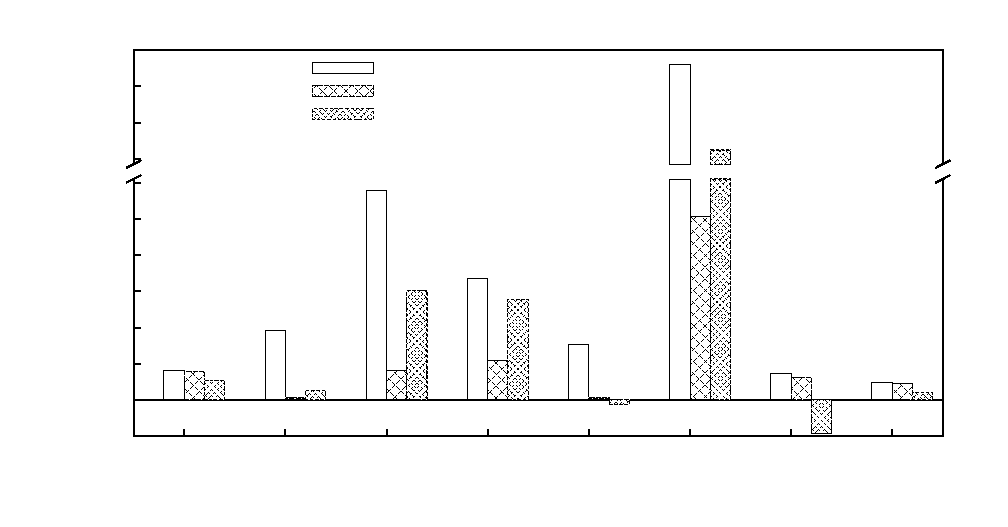
\includegraphics{figures/code_coverage_graph}}%
    \gplfronttext
  \end{picture}%
\endgroup
}
  \caption[Graph of scanner code coverage results.]{Visual representation of the percentage increase of code
    coverage over the baseline scanner, \wget{}. Important to note is
    the gain our scanner, \crawler{}, has over \waf{}, because the
    only difference is our state-aware crawling. The $y$-axis range is
    broken to reduce the distortion of the \wackopicko{} results. }
  \locallabel{code-coverage-graph}
\end{figure}
